% ------------------------------------------------------------------------
% ------------------------------------------------------------------------
% abnTeX2: Modelo de Relatório Técnico/Acadêmico em conformidade com
% ABNT NBR 10719:2011 Informação e documentação - Relatório técnico e/ou
% científico - Apresentação
% ------------------------------------------------------------------------
% ------------------------------------------------------------------------

\documentclass[
	% -- opções da classe memoir --
	12pt,				% tamanho da fonte
%	openright,			% capítulos começam em pág ímpar (insere página vazia caso preciso)
	oneside,			% para impressão em verso e anverso. Oposto a oneside
	a4paper,			% tamanho do papel.
	% -- opções da classe abntex2 --
	%chapter=TITLE,		% títulos de capítulos convertidos em letras maiúsculas
	%section=TITLE,		% títulos de seções convertidos em letras maiúsculas
	%subsection=TITLE,	% títulos de subseções convertidos em letras maiúsculas
	%subsubsection=TITLE,% títulos de subsubseções convertidos em letras maiúsculas
	% -- opções do pacote babel --
	english,			% idioma adicional para hifenização
	french,				% idioma adicional para hifenização
	spanish,			% idioma adicional para hifenização
	brazil,				% o último idioma é o principal do documento
	]{abntex2}


% ---
% PACOTES
% ---

% ---
% Pacotes fundamentais
% ---
\usepackage{cmap}				% Mapear caracteres especiais no PDF
\usepackage{lmodern}			% Usa a fonte Latin Modern
\usepackage[T1]{fontenc}		% Selecao de codigos de fonte.
\usepackage[utf8]{inputenc}		% Codificacao do documento (conversão automática dos acentos)
\usepackage{indentfirst}		% Indenta o primeiro parágrafo de cada seção.
\usepackage{color}				% Controle das cores
\usepackage{graphicx}			% Inclusão de gráficos
% ---

% ---
% Pacotes adicionais, usados no anexo do modelo de folha de identificação
% ---
\usepackage{multicol}
\usepackage{multirow}
% ---

% ---
% Pacotes adicionais, usados apenas no âmbito do Modelo Canônico do abnteX2
% ---
\usepackage{lipsum}				% para geração de dummy text
% ---

% ---
% Pacotes de citações
% ---
\usepackage[brazilian,hyperpageref]{backref}	 % Paginas com as citações na bibl
\usepackage[alf]{abntex2cite}	% Citações padrão ABNT

% ---
% CONFIGURAÇÕES DE PACOTES
% ---

% ---
% Configurações do pacote backref
% Usado sem a opção hyperpageref de backref
\renewcommand{\backrefpagesname}{Citado na(s) página(s):~}
% Texto padrão antes do número das páginas
\renewcommand{\backref}{}
% Define os textos da citação
\renewcommand*{\backrefalt}[4]{
	\ifcase #1 %
		Nenhuma citação no texto.%
	\or
		Citado na página #2.%
	\else
		Citado #1 vezes nas páginas #2.%
	\fi}%
% ---

% ---
% Informações de dados para CAPA e FOLHA DE ROSTO
% ---
\titulo{Relatório Final}
\autor{Saulo Lordão Andrade Barros}
\local{São Cristóvão, Sergipe}
\data{2013}
\instituicao{%
  Universidade Federal de Sergipe -- UFS
  \par
  Departamento de Computação
  \par
  Ciência da Computação
}
\tipotrabalho{Relatório técnico}
% O preambulo deve conter o tipo do trabalho, o objetivo,
% o nome da instituição e a área de concentração
\preambulo{Relatório final referente ao desenvolvimento de um simulador de
processador, como última nota da disciplina de Arquitetura de Computadores no
curso de Graduação em Ciência da Computação.
}
% ---

% ---
% Configurações de aparência do PDF final

% alterando o aspecto da cor azul
\definecolor{blue}{RGB}{41,5,195}

% informações do PDF
\makeatletter
\hypersetup{
		%pagebackref=true,
		pdftitle={\@title},
		pdfauthor={\@author},
		pdfsubject={\imprimirpreambulo},
		pdfcreator={LaTeX with abnTeX2},
		pdfkeywords={abnt}{latex}{abntex}{abntex2}{relatório técnico},
		colorlinks=true,			% false: boxed links; true: colored links
		linkcolor=blue,				% color of internal links
		citecolor=blue,				% color of links to bibliography
		filecolor=magenta,				% color of file links
		urlcolor=blue,
		bookmarksdepth=4
}
\makeatother
% ---

% ---
% Espaçamentos entre linhas e parágrafos
% ---

% O tamanho do parágrafo é dado por:
\setlength{\parindent}{1.3cm}

% Controle do espaçamento entre um parágrafo e outro:
\setlength{\parskip}{0.2cm}  % tente também \onelineskip

% ---
% compila o indice
% ---
\makeindex
% ---

% ----
% Início do documento
% ----
\begin{document}

% Retira espaço extra obsoleto entre as frases.
\frenchspacing

% ----------------------------------------------------------
% ELEMENTOS PRÉ-TEXTUAIS
% ----------------------------------------------------------
% \pretextual

% ---
% Capa
% ---
\imprimircapa
% ---

% ---
% Folha de rosto
% (o * indica que haverá a ficha bibliográfica)
% ---
\imprimirfolhaderosto*
% ---

% ---
% Anverso da folha de rosto:
% ---

{
%\ABNTEXchapterfont

%\vspace*{\fill}

%Conforme a ABNT NBR 10719:2011, seção 4.2.1.1.1, o anverso da folha de rosto
%deve conter:

%\begin{alineas}
%  \item nome do órgão ou entidade responsável que solicitou ou gerou o
%   relatório;
%  \item título do projeto, programa ou plano que o relatório está relacionado;
%  \item título do relatório;
%  \item subtítulo, se houver, deve ser precedido de dois pontos, evidenciando a
%   sua subordinação ao título. O relatório em vários volumes deve ter um título
%   geral. Além deste, cada volume pode ter um título específico;
%  \item número do volume, se houver mais de um, deve constar em cada folha de
%   rosto a especificação do respectivo volume, em algarismo arábico;
%  \item código de identificação, se houver, recomenda-se que seja formado
%   pela sigla da instituição, indicação da categoria do relatório, data,
%   indicação do assunto e número sequencial do relatório na série;
%  \item classificação de segurança. Todos os órgãos, privados ou públicos, que
%   desenvolvam pesquisa de interesse nacional de conteúdo sigiloso, devem
%    informar a classificação adequada, conforme a legislação em vigor;
%  \item nome do autor ou autor-entidade. O título e a qualificação ou a função
%   do autor podem ser incluídos, pois servem para indicar sua autoridade no
%   assunto. Caso a instituição que solicitou o relatório seja a mesma que o
%   gerou, suprime-se o nome da instituição no campo de autoria;
%  \item local (cidade) da instituição responsável e/ou solicitante; NOTA: No
%   caso de cidades homônimas, recomenda-se o acréscimo da sigla da unidade da
%   federação.
%  \item ano de publicação, de acordo com o calendário universal (gregoriano),
%  deve ser apresentado em algarismos arábicos.
%\end{alineas}

%\vspace*{\fill}
%}

% ---
% Agradecimentos
% ---
%\begin{agradecimentos}
%O agradecimento principal é direcionado a Youssef Cherem, autor do
%\nameref{formulado-identificacao} (\autopageref{formulado-identificacao}).

%Os agradecimentos especiais são direcionados ao Centro de Pesquisa em
%Arquitetura da Informação\footnote{\url{http://www.cpai.unb.br/}} da Universidade de
%Brasília (CPAI), ao grupo de usuários
%\emph{latex-br}\footnote{\url{http://groups.google.com/group/latex-br}} e aos
%novos voluntários do grupo
%\emph{\abnTeX}\footnote{\url{http://groups.google.com/group/abntex2} e
%\url{http://abntex2.googlecode.com/}}~que contribuíram e que ainda
%contribuirão para a evolução do abn\TeX.

%\end{agradecimentos}
% ---

% ---
% RESUMO
% ---

% resumo na língua vernácula (obrigatório)
\setlength{\absparsep}{18pt} % ajusta o espaçamento dos parágrafos do resumo
\begin{resumo}
 O domínio dos conceitos de Arquitetura de Computadores é crucial para a
 formação de um Cientista da Computação. Com este trabalho objetiva-se melhorar
 o entendimento do aluno sobre o funcionamento de um processador além de
 introduzi-lo a um projeto de uma arquitetura de processador.

 \noindent
 \textbf{Palavras-chaves}: arquitetura de computadores. simulador de processador.
\end{resumo}
% ---

% ---
% inserir lista de ilustrações
% ---
%\pdfbookmark[0]{\listfigurename}{lof}
%\listoffigures*
%\cleardoublepage
% ---

% ---
% inserir lista de tabelas
% ---
\pdfbookmark[0]{\listtablename}{lot}
\listoftables*
\cleardoublepage
% ---

% ---
% inserir lista de abreviaturas e siglas
% ---
%\begin{siglas}
%  \item[Fig.] Area of the $i^{th}$ component
%  \item[456] Isto é um número
%  \item[123] Isto é outro número
%  \item[lauro cesar] este é o meu nome
%\end{siglas}
% ---

% ---
% inserir lista de símbolos
% ---
%\begin{simbolos}
%  \item[$ \Gamma $] Letra grega Gama
%  \item[$ \Lambda $] Lambda
%  \item[$ \zeta $] Letra grega minúscula zeta
%  \item[$ \in $] Pertence
%\end{simbolos}
% ---

% ---
% inserir o sumario
% ---
\pdfbookmark[0]{\contentsname}{toc}
\tableofcontents*
\cleardoublepage
% ---


% ----------------------------------------------------------
% ELEMENTOS TEXTUAIS
% ----------------------------------------------------------
\textual

% ----------------------------------------------------------
% Introdução
% ----------------------------------------------------------
\chapter*[Introdução]{Introdução}
\addcontentsline{toc}{chapter}{Introdução}
O presente trabalho é a conclusão da disciplina de Arquitetura de Computadores,
ministrada pelo Prof. Marco Túlio Chella, na qual foi demonstrado o
funcionamento e as unidades de processadores, inspirando-se principalmente na
arquitetura Von Neumann.

Para consolidar tais conhecimentos, foi requisitado este trabalho como última
nota da disciplina. O objetivo é desenvolver um sistema computacional com
processador e memória, desde o projeto da arquitetura até a implementação de um
simulador do sistema, a fim de simular fielmente o funcionamento de um
processador, analisando as operações a cada ciclo de \textit{clock}. O simulador de
processador descrito se chama \textbf{Simula-CPU} (implementado em Java),
baseado no processador hipotético \textbf{CPU(12237514)}, criado pelo autor para este
trabalho.


% ----------------------------------------------------------
% PARTE - preparação da pesquisa
% ----------------------------------------------------------
\chapter[Planejamento do Simulador]{Planejamento do simulador}
\section{Pré-Projeto}
Foram poucas as mudanças conceituais entre o projeto final e o pré-projeto. As
unidades continuam sendo as mesmas (e com as mesmas funções), havendo apenas a
inclusão de um decodificador e a ampliação da memória, devido a uma
reestruturação da palavra. Ainda houve algumas mudanças no conjunto de
instruções e no funcionamento de algumas.

\section{Unidades do sistema}

\begin{figure}[htb]
 \label{fig:diagrama-blocos}
 \centering
 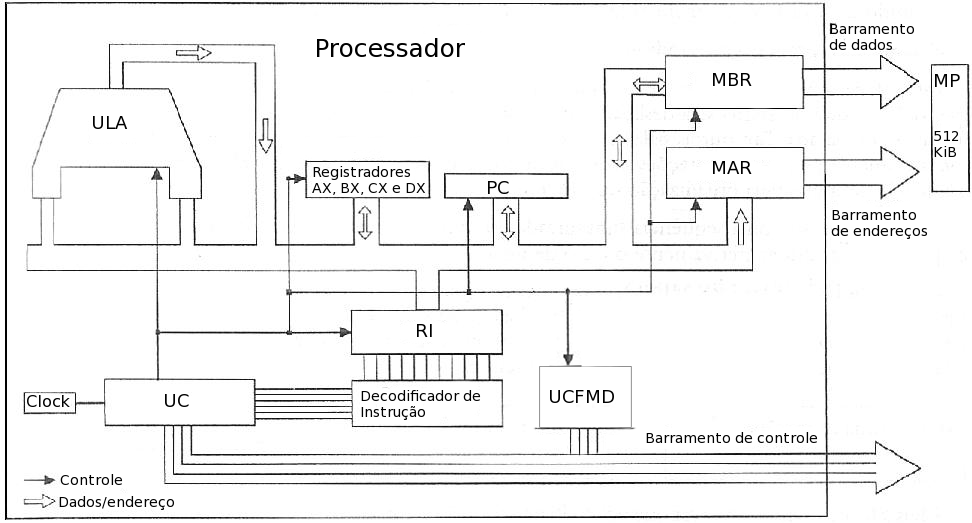
\includegraphics[scale=0.5]{processador.png}
 \legend{Fonte: Adaptado de \cite{monteiro01}}
\end{figure}
	\subsection{Memória}
	A memória do sistema utiliza palavras de 16 bits, armazenando tanto números
	positivos quanto números negativos (a partir do complemento de dois). Há
	capacidade para 32768 palavras de 16 bits, totalizando 512KiB de memória.

	\subsection{Barramentos}
	Há três barramentos: Controle, Dados e Endereço. Toda a comunicação entre
	Processador e Memória é feita através destes três barramentos.

	\subsection{Processador}
		\subsubsection{Registradores}
		O processador possui 8 registradores de 16 bits, implementados com o
		tipo \textit{short}. Destes, quatro são acessíveis ao programador.
		\begin{alineas}
			\item
				AX - Registrador acessível ao programador;
			\item
				BX - Registrador acessível ao programador;
			\item
				CX - Registrador acessível ao programador;
			\item
				DX - Registrador acessível ao programador;
			\item
				PC - Contador de Programa;
			\item
				IR - Registrador de Instrução;
			\item
				MAR - Memory Adress Register. Funciona como buffer dos
				endereços trocados entre o processador e o barramento;
			\item
				MBR - Memory Buffer Register. Funciona como buffer dos
				dados trocados entre o processador e o barramento;
		\end{alineas}

		\subsubsection{Unidade de Controle de Fluxo e de Movimento de Dados}
		Responsável por executar todas as operações que envolvam fluxo do
		programa ou movimento de dados. Encapsula ainda o decodificador de
		instrução;
		\subsubsection{Decodificador}
		Decodifica a instrução recebida, analisando se necessita de operando e
		qual o tipo de operando utilizado por ela;
		\subsubsection{ULA}
		Responsável por todas as operações lógico-aritméticas. Possui um
		registrador de estado, que armazena os estados "Operandos Iguais",
		"Resultado Negativo"~ e "Resultado Zero".


\section{Instruções}
Devido a restrições da linguagem (ausência de tipos sem sinal), o bit mais
significativo não foi utilizado para a definição das instruções, utilizando
sempre o \textit{bit}~imediatamente após o \textit{bit}~de sinal. A construção
das instruções se deu da seguinte forma: O primeiro bit utilizado serve como
\textit{flag}, informando se é instrução lógico-aritmética ou de controle de
fluxo ou de movimento de dados.

No caso de instruções lógico-aritméticas, os dois \textit{bits}~seguintes
indicam se o operando correspondente será um registrador ou um endereço de
memória. Neste simulador só foi implementado o uso de registradores, com estes
dois \textit{bits}~de \textit{flag}~sendo mantidos apenas para facilitar a
implementação desta funcionalidade em outro momento.

Quando a instrução não for lógico-aritmética, o segundo \textit{bit}~indicará se a
instrução é um tipo de MOV. Os três \textit{bits}~restantes indicarão a instrução de
fato.

\begin{table}[htb]
\IBGEtab{%
	\caption{Instruções do processador CPU(12237514)}
	\label{tabela-instrucoes}
}{%
\begin{tabular}{ccc}
\toprule
Código & Mnemônico & Funcionamento \\
\midrule \midrule
000000 & ADD \%AX, \%BX & AX := AX + BX \\
\midrule
000001 & SUB \%AX, \%BX & AX := AX - BX \\
\midrule
000010 & MUL \%AX, \%BX & CX:DX := AX * BX\\
\midrule
000011 & DIV \%AX, \%BX & CX:DX := AX / BX \\
\midrule
000100 & NOT \%AX &  AX := ~AX \\
\midrule
000101 & AND \%AX, \%BX & AX := AX \& BX\\
\midrule
000110 & OR \%AX, \%BX & AX := AX | BX \\
\midrule
000111 & XOR \%AX, \%BX & AX \^ BX \\
\midrule
00000 & NOP & Consome um ciclo de \textit{clock}. \\
\midrule
00001 & JMP \$<end> & PC := <end> \\
\midrule
00010 & JZ & se ULA.estadoVazio(): PC := PC + 2 \\
\midrule
00011 & JNZ & se não ULA.estadoVazio(): PC := PC + 2 \\
\midrule
00100 & JE & se ULA.operandosIguais(): PC := PC + 2 \\
\midrule
00101 & JNE & se não ULA.operandosIguais(): PC := PC + 2 \\
\midrule
00110 & JNG & se ULA.resultadoNegativo(): PC := PC + 2 \\
\midrule
00111 & HLT & Encerra o simulador \\
\midrule
01000 & MOV \%AX, \%BX & AX := BX \\
\midrule
01001 & MOV \%AX, \$<end> & AX := Memoria[<end>] \\
\midrule
01010 & MOV \%AX, \#<valor> & AX := <valor> \\
\midrule
01011 & MOV \$<end>, \%AX & Memoria[<end>] := AX \\
\midrule
01100 & MOV \$<end>, \#<valor> & Memoria[<end>] := <valor> \\
\bottomrule
\end{tabular}%
}{%
	\fonte{Produzido pelos autores.}%
}
\end{table}

\section{Implementação}
O Simula-CPU foi desenvolvido na linguagem de programação Java. Para
representar os dados internos foram utilizados números inteiros, enquanto
a memória utiliza um vetor de inteiros. Cada unidade descrita acima foi
implementada em uma classe própria, aproveitando o paradigma de Orientação a
Objetos.

Os barramentos foram implementados como objetos Singleton, possuindo apenas um
barramento de cada tipo, acessíveis através de métodos estáticos. Estratégias
similares foram usadas nas classes de Memória e Processador. É importante notar
que todas as unidades internas ao processador não são vistas fora do "pacote"~
onde estão, encapsulando o funcionamento destas.

Para facilitar o teste do Simula-CPU, há um tradutor de uma linguagem Assembly
para inteiros, de forma que o processador possa entender o programa escrito.
Este tradutor é responsável também por montar o programa para a memória. Dadas
as funções, esta estrutura foi chamada de Montador, estando em sua própria
classe.

% ----------------------------------------------------------
% Capitulo com exemplos de comandos inseridos de arquivo externo
% ----------------------------------------------------------




% ---
% Finaliza a parte no bookmark do PDF, para que se inicie o bookmark na raiz
% ---
\bookmarksetup{startatroot}%
% ---

% ---
% Conclusão
% ---
\chapter*[Conclusão]{Conclusão}
\addcontentsline{toc}{chapter}{Conclusão}
Ao final deste trabalho, foi possível projetar um simples processador e
implementar um simulador do mesmo. O entendimento do funcionamento de um
processador foi atingido, sendo este o objetivo da disciplina. A experiência
foi enriquecedora ao fornecer uma visão de hardware como algo possível de ser
implementado de fato como software.

% ----------------------------------------------------------
% ELEMENTOS PÓS-TEXTUAIS
% ----------------------------------------------------------
\postextual

% ----------------------------------------------------------
% Referências bibliográficas
% ----------------------------------------------------------
\bibliography{ref}

% ----------------------------------------------------------
% Glossário
% ----------------------------------------------------------
%
% Consulte o manual da classe abntex2 para orientações sobre o glossário.
%
%\glossary

% ----------------------------------------------------------
% Apêndices
% ----------------------------------------------------------

% ---
% Inicia os apêndices
% ---
%\begin{apendicesenv}

% Imprime uma página indicando o início dos apêndices
%\partapendices

% ----------------------------------------------------------
%\chapter{Quisque libero justo}
% ----------------------------------------------------------


%\end{apendicesenv}
% ---


% ----------------------------------------------------------
% Anexos
% ----------------------------------------------------------

% ---
% Inicia os anexos
% ---
%\begin{anexosenv}

% Imprime uma página indicando o início dos anexos
%\partanexos



%\end{anexosenv}

%---------------------------------------------------------------------
% INDICE REMISSIVO
%---------------------------------------------------------------------

\printindex


\end{document}
